\section*{Milstein Method}
The \textbf{Milstein}\cite{wiki:milstein} method improves the Euler-Maruyama approximation by adding the second-order term from the Ito-Taylor expansion. This increases the strong convergence order from $0.5$ to $1.0$.
\\
\\
Consider a stochastic differential equation of the form as shown in $\eqref{eq:sde_1}$
The Euler-Maruyama method only keeps the first order terms while Milstein includes an additional term to account for the noise on diffusion signal. Apart from identifying the drift $a(X_t)$ and the diffusion $b(X_t)$, we also need the derivative $b'(X_t)$.
\begin{align*}
f(x) = \mu x\\
g(x) = \sigma x\\
g'(x) = \sigma
\end{align*}
We derive the Milstein method from the diffusion term of $\eqref{eq:sde_1}$ by performing the truncated Taylor expansion of $g(X_t)$ around $X_n$ using Ito's lemma
\begin{align*}
g(X_t) \approx g(X_n) + g^{'}(X_n)(X_t-X_n)
\end{align*}
Substitute $g(X_t)\approx g(X_n)dW_t$ into $g(X_t)dW_t$ integral
\begin{align*}
\int_{t_n}^{t_{n+1}}g(X_s,s)dW_s
\end{align*}
becomes
\begin{align*}
\int_{t_n}^{t_{n+1}} g(X_t)dW_s + \int_{t_n}^{t_{n+1}} g^{'}(X_t,t) (X_s - X_t)dW_s
\end{align*}
We approximate $(X_s - X_t)$ from the diffusion term of \eqref{eq:sde_1} to capture the stochastic behavior
\begin{align*}
X_s - X_t \approx f(X_t,t)(s-t) + g(X_t,t)(W_s-W_t)
\end{align*}
and substitute to the second integral
\begin{align*}
\int_{t_n}^{t_{n+1}} g(X_t)dW_t &\approx \int_{t_n}^{t_{n+1}}\left[g(X_n) + g^{'}(X_n) g(X_n)(W_{t_{n+1}}-W_{t_n})\right]dW_t\\
&\approx \int_{t_n}^{t_{n+1}} g(X_n) dW_s \\ 
&\qquad\qquad + \int_{t_n}^{t_{n+1}} g(X_n)b^{'}(X_n)(W_s-W_{t_n})dW_s\\
&\approx g(X_n) \Delta W_n + g(X_n)g^{'}(X_n) \int_{t_n}^{t_{n+1}} (W_{s} - W_{t_n}) dW_s
\end{align*}
To solve the remaining integral, we use Ito's formula on the process $f(x)=x^2$ applied to $X_s := W_s - W_{t_n}$ for all $s \in [t_n, t_{n+1}]$
We now use $f(x)=f(W_s)=(W_s - W_{t_n})^2$ and by Ito's formula
\begin{align*}
df(W_s) = f'(W_s)dW_s + \frac{1}{2} f"(W_s)dW_s^2 
\end{align*}
Compute the derivatives
\begin{align*}
f'(W_s) &= 2(W_s - W_t)\\
f^{"}(W_s) &= 2\\
(dW_s)^2 &= ds
\end{align*}
Substitute the derivatives to Ito's formula
\begin{align*}
d[(W_s - W_t)^2] &= 2(W_s - W_t) dW_s + \frac{1}{2}(2)ds\\
&= 2(W_s - W_t)dW_s + ds
\end{align*}
Integrate from $t$ to $s$
\begin{align*}
\int_{t}^{s} d(W_s-W_t)^2 &= \int_t^2 2(W_s - W_t)dWs + \int_t^2 ds\\
(W_s - W_t)^2 -(W_{t} - W_t)^2 &= 2 \int_{t}^{s} (W_s - W_t)dW_s + (s - t) \\
(W_s - W_t)^2 &= 2 \int_{t}^{s} (W_s - W_t)dW_s + (s - t)
\end{align*}
Rearranging to find the integral
\begin{align*}
\int_{t}^{s} (W_s - W_t)dW_s &= \frac{1}{2}\left[(W_{s} - W_t)^2 - (s - t)\right] \\
&= \frac{1}{2} (dW_t)^2 - dt
\end{align*}
Combining this extra correction term with the original Euler-Maruyama expression, we get the Milstein method with the added correction term.
\begin{align*}
X_{t_{n+1}} = X_t + f(X_t)dt + g(X_t)dW_t + \frac{1}{2} g'(X_t)g(X_t)\big[(dW_t)^2-dt\big]
\end{align*}
This term specifically targets the SDE's where the diffusion $g(X_t)$ depends on the state $X_t$. If $g(X_t)$ is constant, the derivative $g'(X_t)$ is zero and Milstein method collapses back to Euler-Maruyama.
\begin{figure}[h!]
    \centering    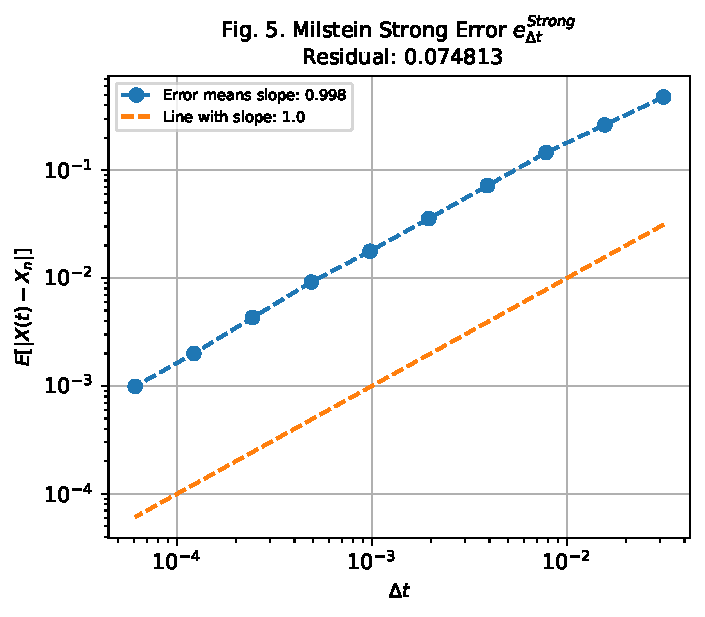
\includegraphics[width=0.5\textwidth]{../figures/milstein_strong_convergence.pdf}
    \caption{Milstein Strong Error Convergence} %
    \label{fig:fig_5}
\end{figure}
We compare the performance of the Milstein method in Fig. \ref{fig:fig_5} with Euler-Maruyama in Fig. \ref{fig:fig_3} with the same Monte-Carlo simulation size and we can confirm improvement of the slope of the means of error. The following Fig. \ref{fig:fig_6} illustrates the Milstein weak error order of $1$ which is normally used where overall distribution is more important when assessing the reliability of the numerical method.
\begin{figure}[h!]
    \centering
    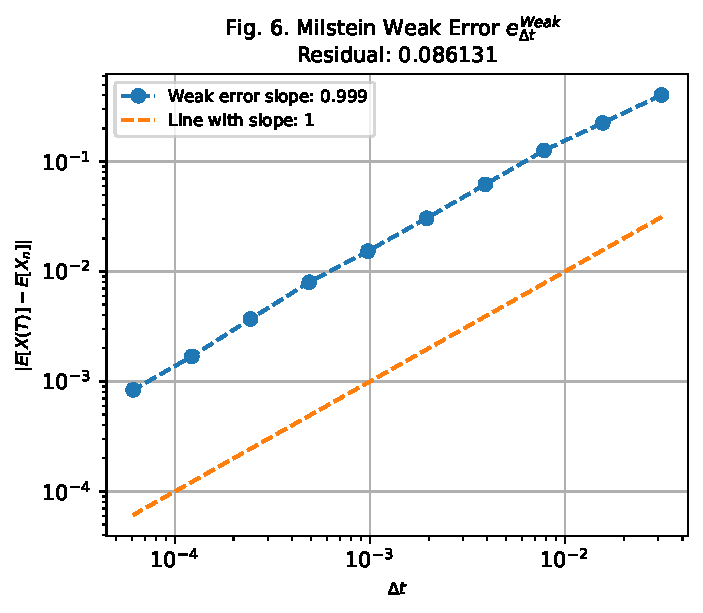
\includegraphics[width=0.5\textwidth]{../figures/milstein_weak_convergence.pdf}
    \caption{Milstein Weak Error Convergence}
    \label{fig:fig_6}
\end{figure}
